\documentclass[12pt,a4paper]{article}

\usepackage[utf8]{inputenc}
\usepackage[T1]{fontenc}
\usepackage[spanish]{babel}
\usepackage[margin=2.2cm]{geometry}
\usepackage{setspace}
\onehalfspacing
\usepackage[sfdefault]{carlito}
\usepackage{graphicx}
\usepackage{hyperref}
\usepackage{xcolor}
\usepackage{amsmath}
\usepackage{enumitem}

\hypersetup{colorlinks=true, linkcolor=blue, urlcolor=blue, citecolor=blue}

\newcommand{\Universidad}{Universidad Internacional de La Rioja (UNIR)}
\newcommand{\Asignatura}{Informática Gráfica y Visualización}

\title{\textbf{Trabajo 7: Proyecciones 3D}\\Cuatro vistas de un mismo cubo en OpenGL}
\author{Sergio Andrés Majé Franco}
\date{\Asignatura \\ \Universidad \\ 28 de mayo de 2026}

\begin{document}

\maketitle
\tableofcontents
\newpage

\section{Introducción}
El Trabajo 7 pide construir una ventana OpenGL con cuatro vistas simultáneas del mismo cubo. Cada vista debe usar una proyección distinta: ortográfica, gabinete, perspectiva simétrica y perspectiva oblicua. Además, el enunciado impone una restricción importante: no se puede mover el ojo desde la posición por defecto $(0,0,0)$, por lo que no se permite utilizar \texttt{gluLookAt()} ni mecanismos equivalentes.

La solución desarrollada mantiene esa restricción de forma estricta. El cubo es el único objeto que se transforma geométricamente para quedar delante del observador. En consecuencia, la comparación entre proyecciones se apoya únicamente en matrices de proyección distintas y en una misma transformación de modelo aplicada a los cuatro cuadrantes.

\section{Planteamiento geométrico}
\subsection{Escena común}
Los cuatro cuadrantes representan exactamente la misma escena:

\begin{itemize}[leftmargin=*]
    \item un cubo centrado en el origen del modelo;
    \item ejes cartesianos simples para dar referencia espacial;
    \item una traslación global sobre el eje $-Z$ para situar el cubo delante del ojo;
    \item rotaciones fijas sobre $X$, $Y$ y $Z$ para que las tres dimensiones sean legibles en todos los casos.
\end{itemize}

La transformación de modelo se mantiene constante. En términos prácticos, el programa aplica una traslación aproximada de $(0,-0.1,-8)$ y después varias rotaciones fijas. Esta decisión hace que cualquier diferencia visual entre cuadrantes provenga de la proyección y no de cambios de cámara o de pose entre vistas.

\subsection{Matrices de proyección}
Las matrices se codifican de forma explícita en \texttt{main.c}. No se delega la construcción de la cámara a utilidades externas. Las cuatro familias empleadas son las siguientes:

\paragraph{Proyección ortográfica.}
Se utiliza la forma clásica de la matriz ortográfica:

\[
O =
\begin{bmatrix}
\frac{2}{r-l} & 0 & 0 & -\frac{r+l}{r-l} \\
0 & \frac{2}{t-b} & 0 & -\frac{t+b}{t-b} \\
0 & 0 & -\frac{2}{f-n} & -\frac{f+n}{f-n} \\
0 & 0 & 0 & 1
\end{bmatrix}
\]

Su efecto visual es conservar paralelas todas las aristas del cubo, sin convergencia hacia puntos de fuga.

\paragraph{Proyección gabinete.}
La vista gabinete se construye combinando una proyección ortográfica con una cizalla sobre el eje de profundidad. En el código se implementa como el producto $O \cdot S$, donde $S$ desplaza $x$ e $y$ proporcionalmente a $z$ con un factor de acortamiento $0.5$ y un ángulo de $45^\circ$. Esto preserva el carácter oblicuo y hace que las aristas de fuga se perciban con media escala, que es la convención habitual del gabinete.

\paragraph{Perspectiva simétrica.}
Se usa una matriz de \emph{frustum} centrada:

\[
P =
\begin{bmatrix}
\frac{2n}{r-l} & 0 & \frac{r+l}{r-l} & 0 \\
0 & \frac{2n}{t-b} & \frac{t+b}{t-b} & 0 \\
0 & 0 & -\frac{f+n}{f-n} & -\frac{2fn}{f-n} \\
0 & 0 & -1 & 0
\end{bmatrix}
\]

En este caso se cumple $l = -r$ y $b = -t$, de modo que el volumen de visión es simétrico.

\paragraph{Perspectiva oblicua asimétrica.}
Para la cuarta vista se reaprovecha la misma familia de matriz de \emph{frustum}, pero con límites laterales y verticales no simétricos. Así aparece una perspectiva desplazada lateralmente, que rompe la alineación central y genera una sensación oblicua sin mover el ojo.

\section{Implementación}
\subsection{Estructura del programa}
Todo el trabajo queda contenido en \texttt{main.c}, como pedía el enunciado. La lógica principal se divide en cuatro bloques:

\begin{itemize}[leftmargin=*]
    \item creación de la ventana X11 y del contexto GLX;
    \item construcción explícita de las matrices de proyección;
    \item renderizado del cubo en cuatro \emph{viewports} dentro de una sola ventana;
    \item gestión de eventos de cierre, teclado y redimensionado.
\end{itemize}

El uso de \emph{viewports} permite reutilizar la misma geometría sin duplicar escenas. Cada cuadrante limpia su propio fondo, carga su matriz de proyección y renderiza el cubo con la misma transformación de modelo. Después se dibujan divisores en pantalla para reforzar la lectura visual en la captura.

\subsection{Decisiones de representación}
Se han tomado varias decisiones para que la comparación entre proyecciones resulte clara:

\begin{itemize}[leftmargin=*]
    \item las caras del cubo están coloreadas para distinguir su orientación;
    \item las aristas se dibujan encima de las caras para reforzar la percepción de volumen;
    \item los ejes se añaden como referencia espacial mínima;
    \item cada cuadrante usa un fondo ligeramente distinto, pero muy cercano, para separar visualmente las vistas sin distraer.
\end{itemize}

\subsection{Restricción sobre la posición del ojo}
El código no usa \texttt{gluLookAt()} ni ninguna rutina equivalente de cámara. La escena parte siempre del ojo por defecto y el cubo es el que se traslada hacia el eje $-Z$. Esto responde de forma directa a la condición explícita del trabajo.

\section{Resultado}
\subsection{Captura del programa}
\IfFileExists{../captures/proyecciones-3d.png}{%
    \begin{center}
    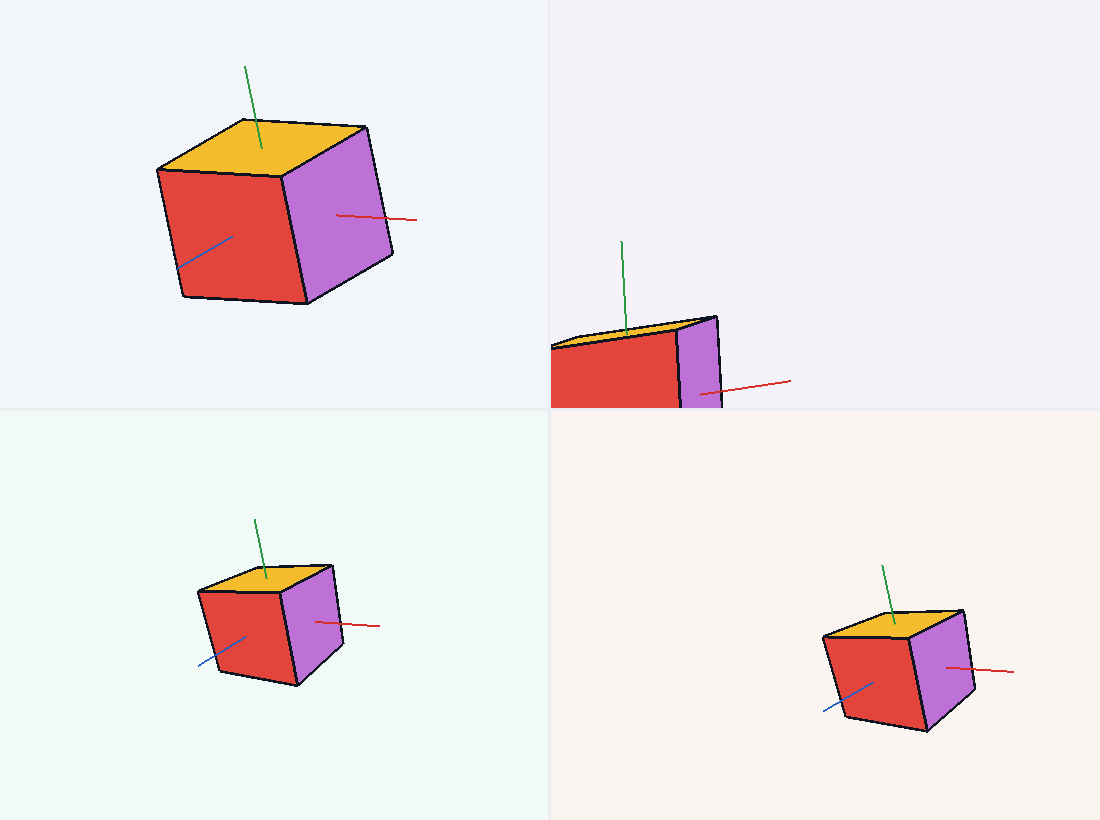
\includegraphics[width=0.96\textwidth]{../captures/proyecciones-3d.png}
    \end{center}
}{%
    \fcolorbox{black}{gray!10}{%
        \parbox{0.9\textwidth}{%
            Captura pendiente de incorporar en \texttt{captures/proyecciones-3d.png}.
        }%
    }%
}

\smallskip

\textbf{Figura 1.} Ventana del Trabajo 7 con las cuatro proyecciones simultáneas.

\subsection{Funcionamiento}
\textbf{¿Funciona bien tu programa?}

Sí. El programa abre una única ventana OpenGL y muestra de forma estable las cuatro vistas solicitadas. La escena se mantiene coherente durante el redimensionado y cada cuadrante presenta un comportamiento visual compatible con la familia de proyección que le corresponde. La ortográfica mantiene el paralelismo, la gabinete conserva profundidad oblicua con acortamiento, la perspectiva simétrica produce convergencia centrada y la perspectiva oblicua asimétrica desplaza ese volumen de visión.

\section{Limitaciones y fallos detectados}
\textbf{¿Qué fallos existen?}

La solución cumple el objetivo del trabajo, pero conviene dejar documentadas varias limitaciones:

\begin{itemize}[leftmargin=*]
    \item depende de un entorno gráfico con X11/GLX y OpenGL clásico, por lo que no es una solución nativa para Windows sin WSL o sin un servidor X;
    \item no incluye texto rotulado dentro de cada cuadrante, por lo que la identificación de vistas se apoya en el orden documentado y en el informe;
    \item los valores numéricos elegidos para cada matriz se han ajustado manualmente para priorizar legibilidad sobre generalidad;
    \item la perspectiva oblicua se resuelve como un \emph{frustum} asimétrico, que es una interpretación defendible del requisito, aunque el enunciado no fija una parametrización única para esa cuarta proyección.
\end{itemize}

\section{Rescate de Cálculo Vectorial}
Como ampliación del repositorio se ha incorporado un proyecto independiente. Su ubicación es \texttt{extras/calculo-vectorial-figura-1/}. Este extra no forma parte de la entrega principal del Trabajo 7, pero recupera la Figura 1 del laboratorio previo de Cálculo Vectorial dentro del mismo entorno técnico de OpenGL clásico.

La superficie representada viene dada por la ecuación:

\[
\frac{x^2}{9} + \frac{(y-3)^2}{4} - \frac{(z+1)^2}{9} = 1
\]

Se trata de un hiperboloide de una hoja centrado en $(0, 3, -1)$ y orientado a lo largo del eje $z$. En el programa se parametriza mediante funciones hiperbólicas:

\[
x = 3 \cosh(v) \cos(u), \quad
y = 3 + 2 \cosh(v) \sin(u), \quad
z = -1 + 3 \sinh(v)
\]

con $u \in [0, 2\pi]$ y un rango acotado de $v$ para muestrear una banda visible de la superficie. La representación se dibuja como malla alámbrica, lo que reduce complejidad visual y conserva claridad geométrica.

\IfFileExists{../../../extras/calculo-vectorial-figura-1/captures/figura1.png}{%
    \begin{center}
    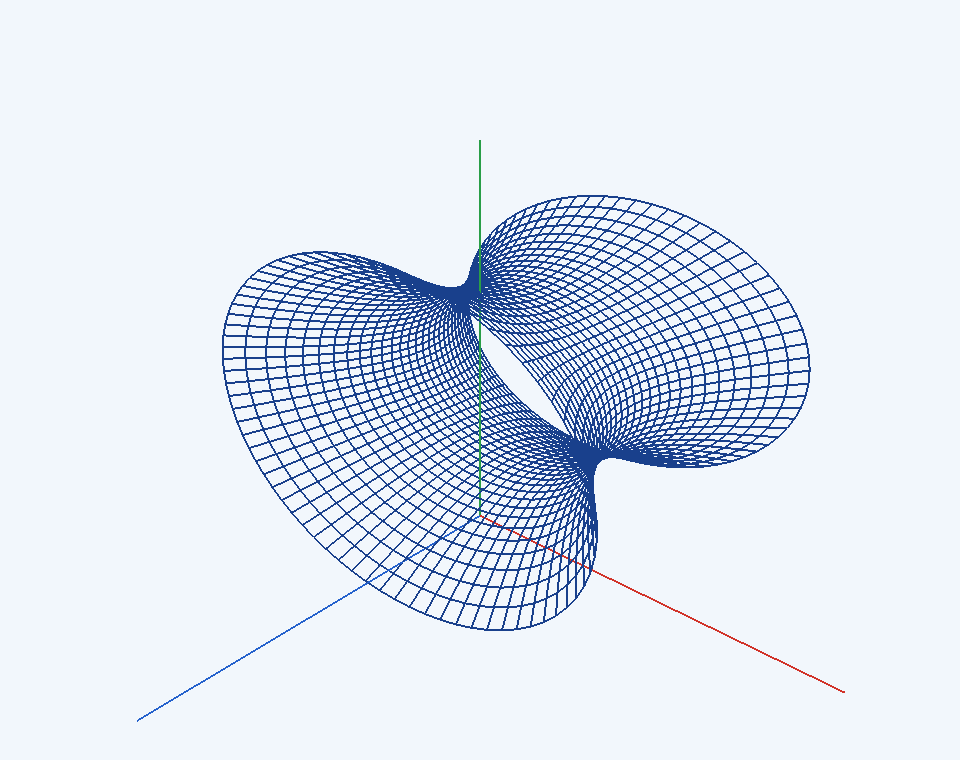
\includegraphics[width=0.72\textwidth]{../../../extras/calculo-vectorial-figura-1/captures/figura1.png}
    \end{center}
}{}

\smallskip

Este rescate aporta valor al repositorio porque reutiliza la misma infraestructura gráfica de la asignatura para representar otra superficie relevante, pero sin mezclarla con la práctica principal.

\section{Conclusiones}
El trabajo resuelve de forma directa la comparación entre distintas proyecciones 3D sobre una misma geometría, que es precisamente el foco del Tema 7. La implementación es sencilla de defender porque separa con claridad la escena común de las matrices de proyección y evita dependencias de cámara que contradigan el enunciado.

Además, la nueva estructura del repositorio deja el laboratorio del reloj como antecedente histórico, incorpora el Trabajo 7 como práctica principal y añade un extra matemático reutilizable. El resultado es un monorepo más ordenado, más fácil de mantener y con mejor continuidad técnica entre ejercicios.

\section{Formato de entrega}
El informe se mantiene en LaTeX y se genera a PDF dentro del repositorio. Esto deja documentado el trabajo de forma reproducible, aunque la nota del enunciado indicaba expresamente que sólo se aceptaban formatos editables y no PDF.

\end{document}
